\RequirePackage{luatex85}
\PassOptionsToPackage{shorthands=off}{babel}
\makeatletter
\disable@package@load{fontenc}
\makeatother
\let\oldlooseness=\looseness
\documentclass{csbulletin}
\selectlanguage{czech}
\usepackage{titlesec}
\titlelabel{\thetitle\enspace}
\usepackage{luavlna}
\usepackage[strict]{lua-widow-control}
\usepackage{csquotes}
\usepackage[
  backend=biber,
  citestyle=numeric-comp,
  bibstyle=iso-numeric,
  sortlocale=cs,
  autolang=other,
  bibencoding=UTF8,
  mincitenames=2,
  maxcitenames=2,
  doi=true,
  isbn=true,
  shortnumeration=true,
]{biblatex}
\renewcommand\multicitedelim{\addsemicolon\space}
\addbibresource{starynovotny-tug2024.bib}
\usepackage[
  implicit=false,
  hidelinks,
]{hyperref}
\usepackage{hologo}

\newcommand\acro[1]{\textsc{\MakeLowercase{#1}}}
\newcommand\pkg{\textsf}
\makeatletter
\DeclareRobustCommand{\La}{L\kern-.36em%
        {\sbox\z@ T%
         \vbox to\ht\z@{\hbox{\check@mathfonts
                              \fontsize\sf@size\z@
                              \math@fontsfalse\selectfont
                              A}%
                        \vss}%
        }}
\def\strankasclankem#1#2{%
  \begingroup
  \def\csbul@start@page##1{%
    ##1%
    \endinput
    \ignorespaces
  }%
  \makeatletter
  \IfFileExists{../#1/#2.info}{\input ../#1/#2.info\relax}{\textbf{???}}%
  \endgroup
}
\makeatother
\def\AllTeX{(\La\kern-.075em)\kern-.075em\TeX}

\begin{document}

\singlechars{czech}{AaIiVvOoUuSsZzKk}

\title{\CSTUG{} na konferenci TUG 2024}
\EnglishTitle{\CSTUG{} at the TUG 2024 Conference}
\author{Vít Starý Novotný, Michal Hoftich, Jaromír Kuben}
\podpis{Vít Starý Novotný, witiko@mail.muni.cz
     \\ Michal Hoftich, michal.h21@gmail.com
     \\ Jaromír Kuben, jaromir.kuben@unob.cz}
\maketitle

Od čtvrtka 18.\,července do neděle 21.\,července se v Praze s podporou sdružení \CSTUG{} konala konference TUG 2024. S organizací konference pomohl předseda Petr Sojka, jeho syn Ondřej a členové výboru \CSTUG u Michal Hoftich a Jaromír Kuben. Konference se také aktivně zúčastnil Vítek Starý Novotný. Dorazilo téměř 60 účastníků, kromě zástupců evropských států a \acro{USA} také početná skupina z Indie, kam se konference příští rok přesune.
\medskip

Ve čtvrtek ještě před oficiálním zahájením konference proběhl v prostorách \acro{MFF UK} tutoriál věnovaný tvorbě značkovaných \acro{PDF} dokumentů.
Tutoriál moderovala Ulrike Fischer, členka týmu \LaTeX, který se tímto projektem již delší dobu zabývá~\cite{mittelbach2022latex}. Účastníci se dozvěděli, které z často užívaných balíčků už podporují vytváření dobře značkovaných dokumentů a které jsou na seznamu čekatelů o doplnění této schopnosti.

V pátek dopoledne ukázal Martin Ruckert v přednášce nazvané \emph{\foreignlanguage{english}{Profiling \TeX{} input files}}~\cite{ruckert2024profiling} nástroje \texttt{texprof} a \texttt{texprofile}, pomocí kterých je možné měřit rychlost kódu v \TeX u. Překlad článku z přednášky začíná na straně \strankasclankem{Ruckert-profiling}{ruckert-profiling}.

Stejný den odpoledne ukázal Vítek Starý Novotný v přednášce nazvané \emph{\foreignlanguage{english}{Markdown themes in practice}}~\cite{starynovotny2024markdowna, starynovotny2024markdownc}, jak je možné generovat testové otázky na základě souborů ve formátu \acro{YAML} a Markdown, vizte Obrázek~\ref{fig:vitek}.

\begin{figure}[p]
\centering
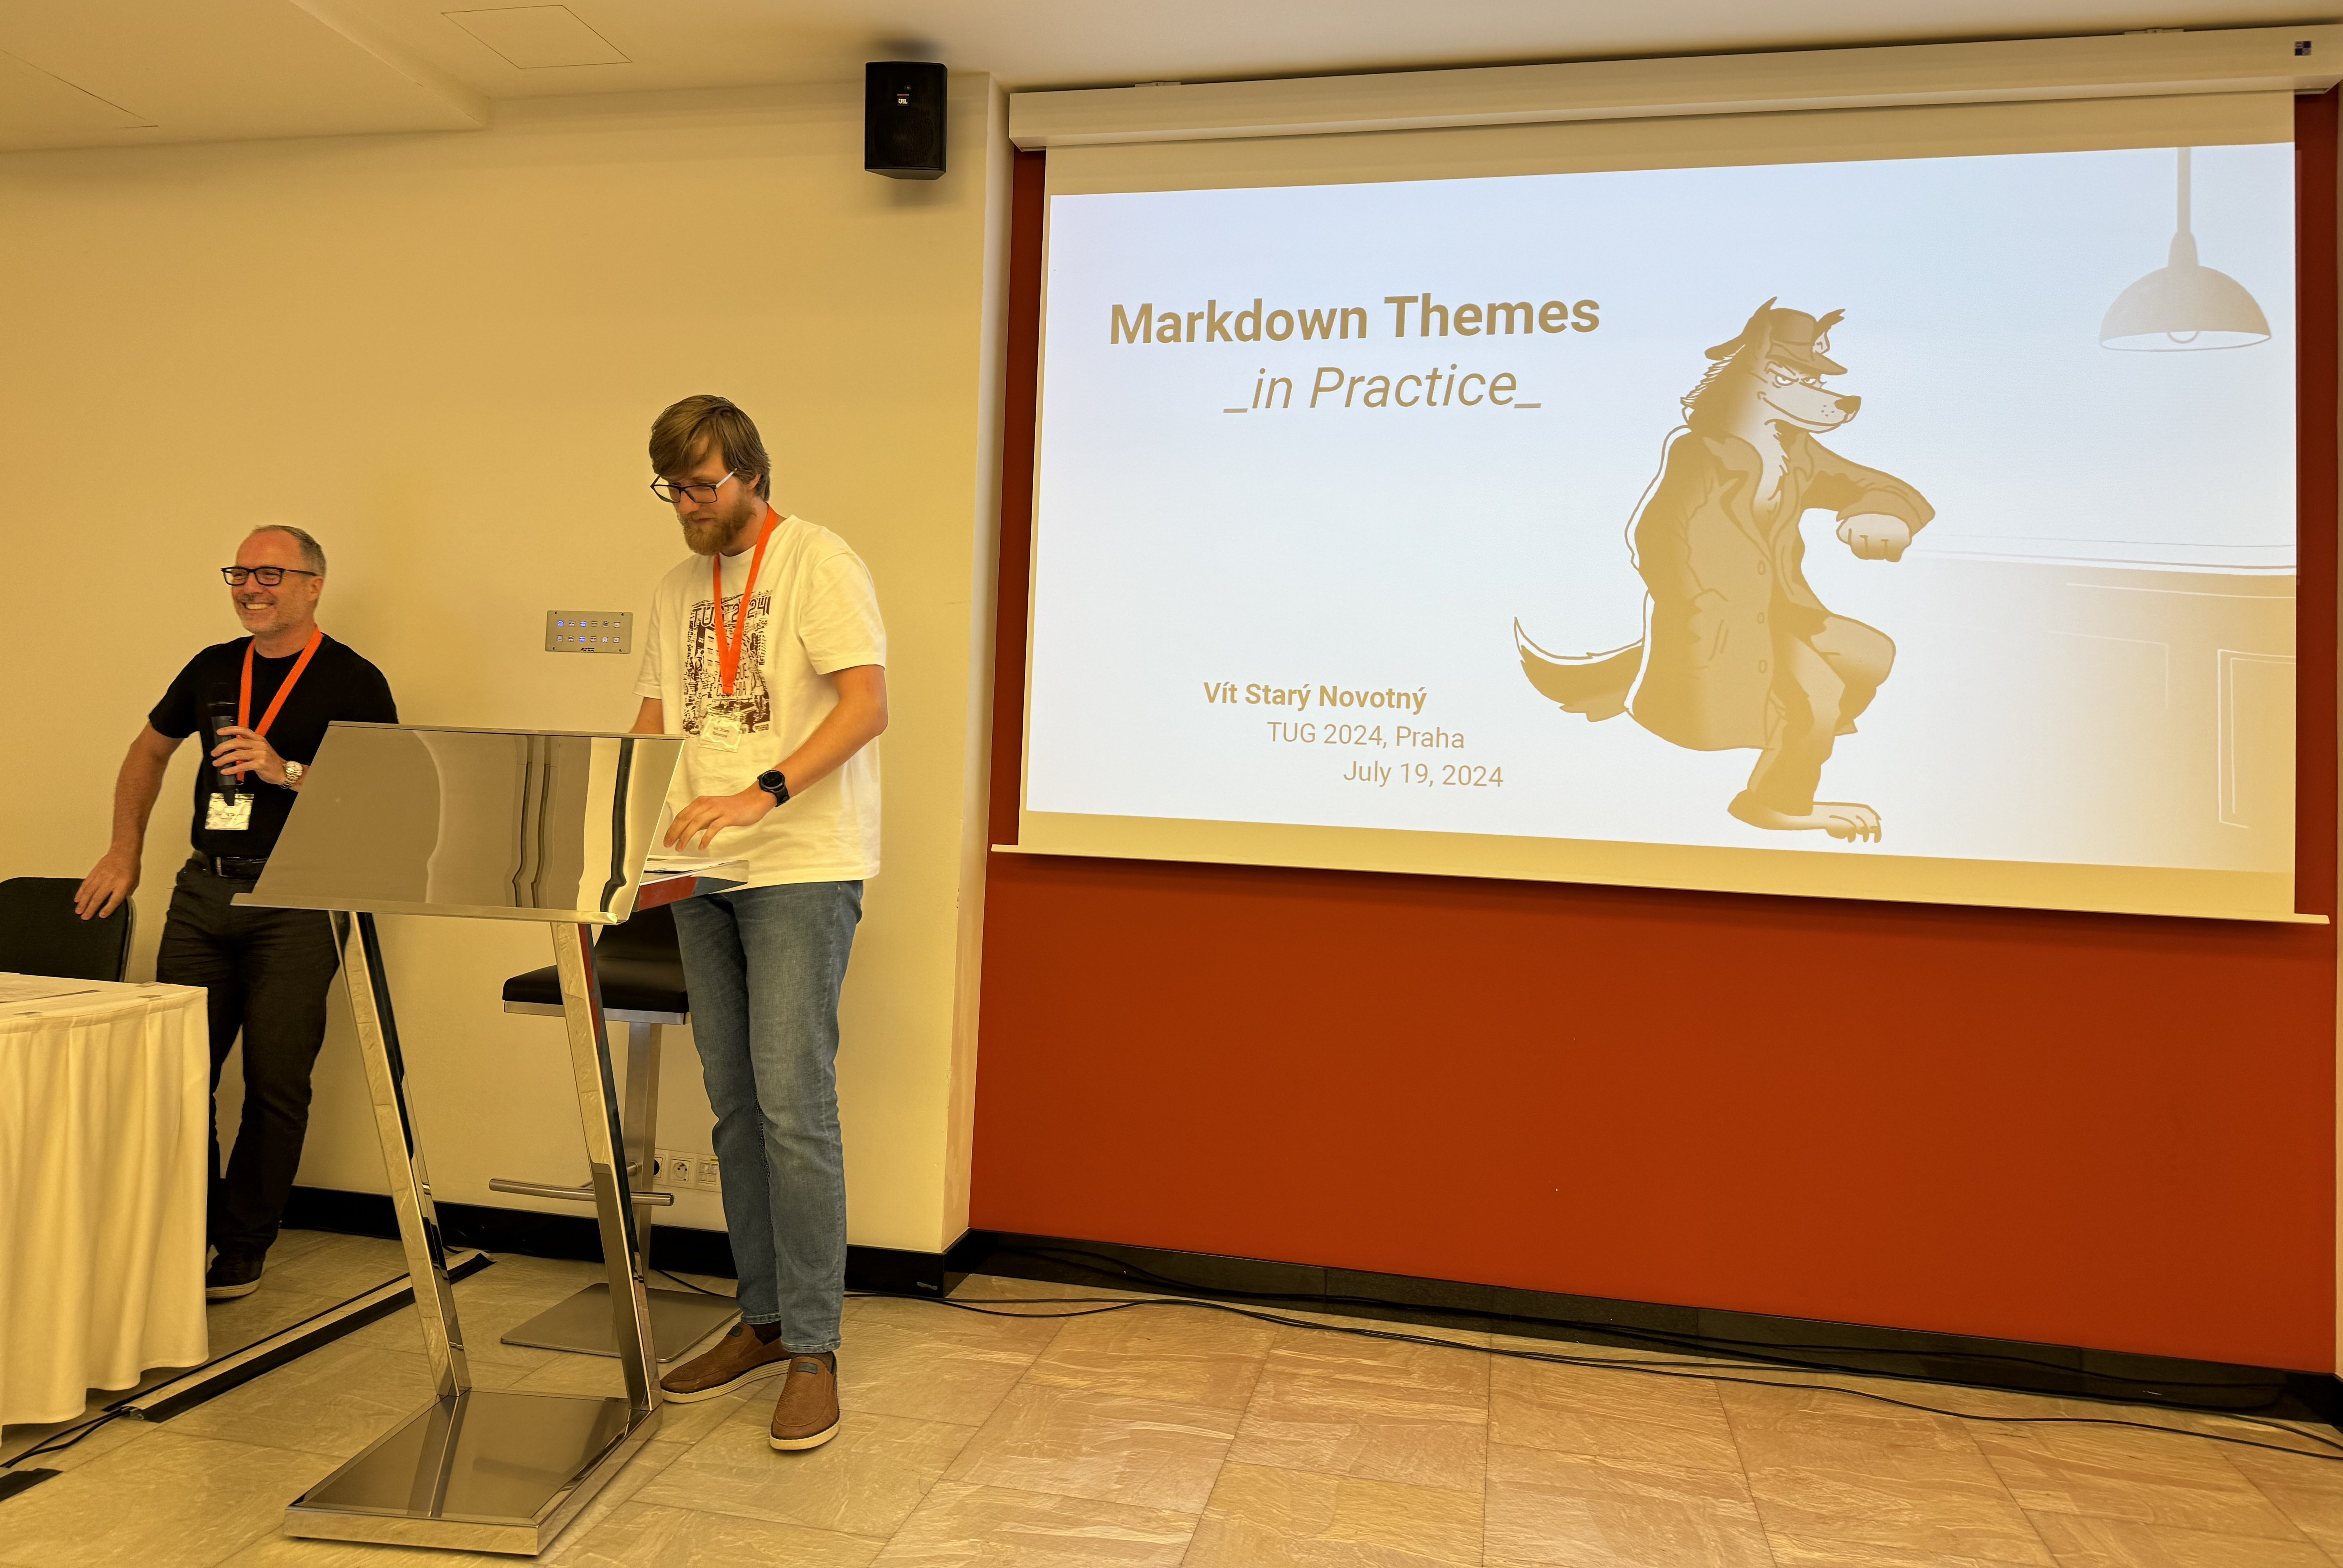
\includegraphics[width=\linewidth]{figs/vitek-pred-prednaskou}\par\medskip
\fboxsep=0pt\kern-\fboxrule\relax\fbox{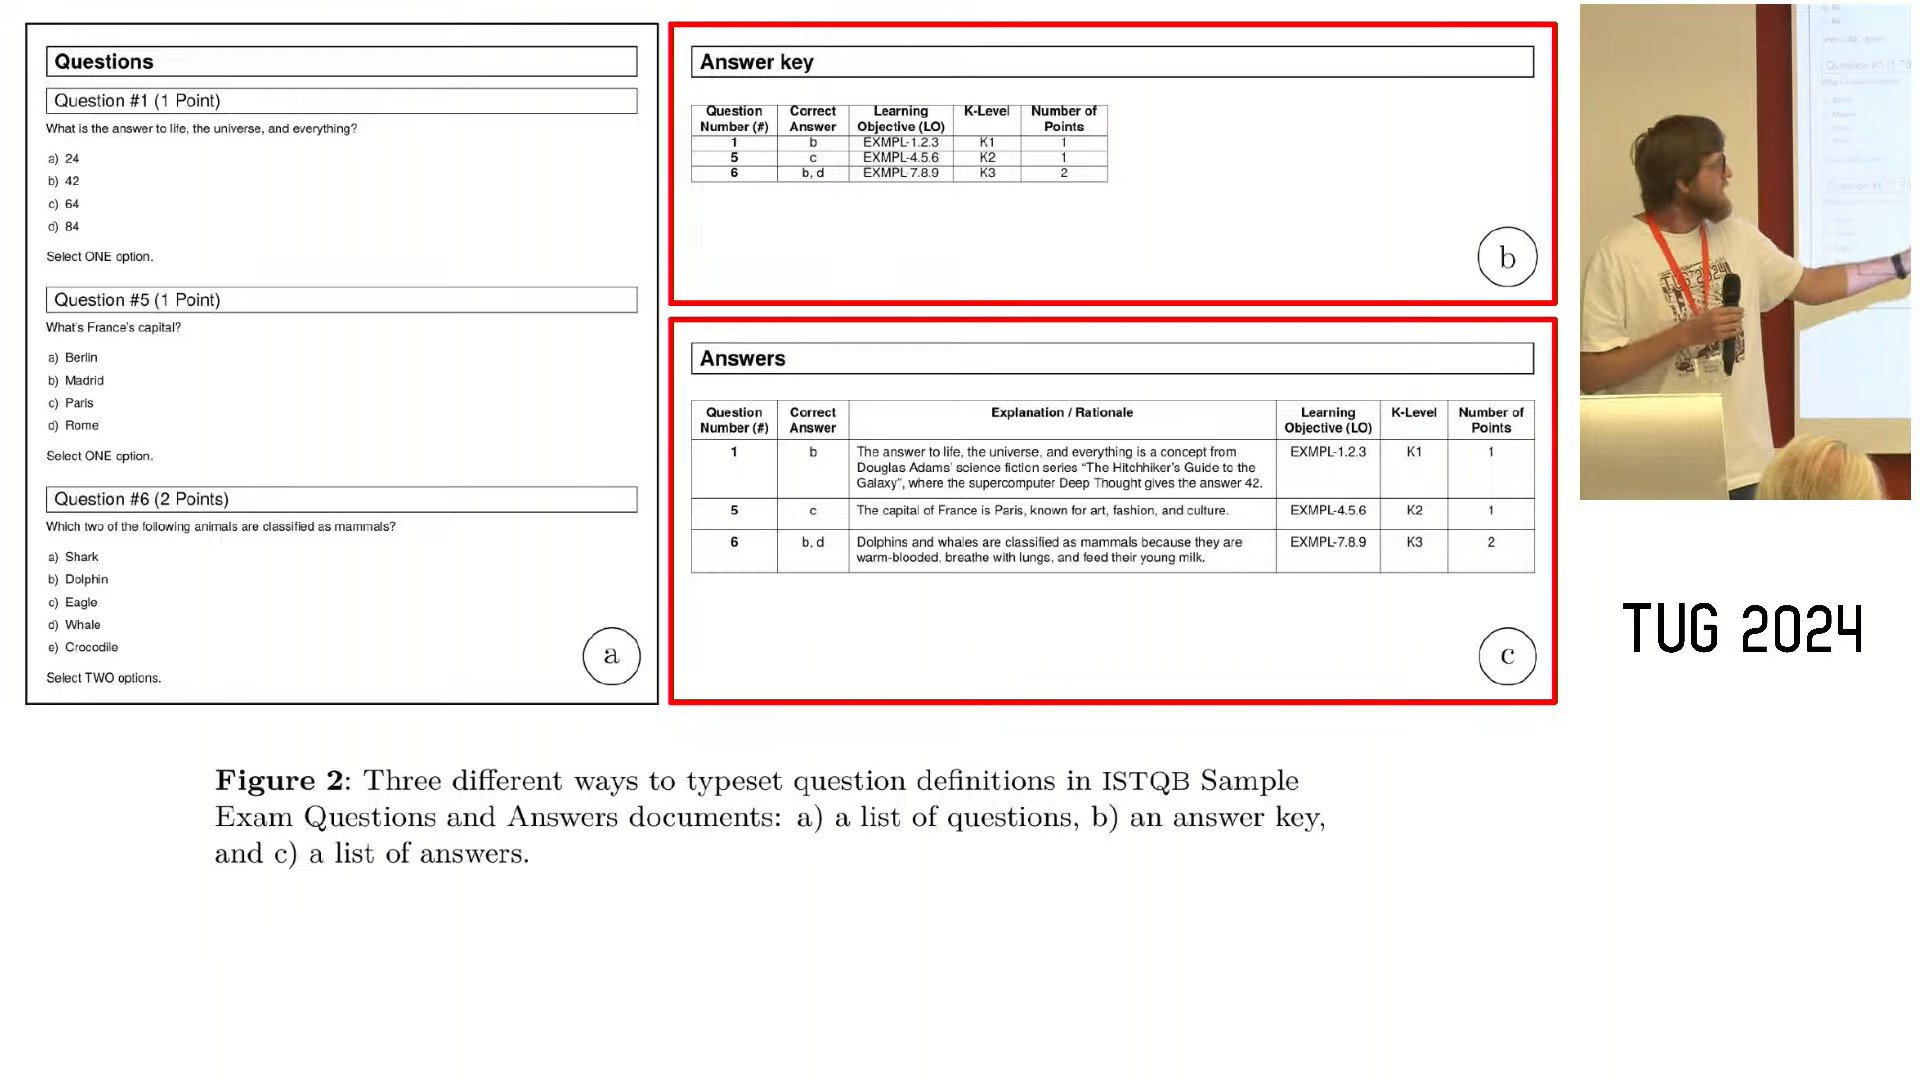
\includegraphics[width=\linewidth]{figs/vitek-behem-prednasky}}%
\caption{Vítek Starý Novotný přednáší o generování testových otázek na základě souborů ve formátech \acro{YAML} a Markdown.}
\label{fig:vitek}
\end{figure}

Téhož dne večer ukázali Oliver Kopp, Marcel Krüger a Marei Peischl na workshopu nazvaném \emph{\foreignlanguage{english}{Creation of \LaTeX{} documents using a cloud-based pipeline}}~\cite{peischl2024pipeline}, jak je možné vytvářet \AllTeX ové dokumenty v cloudu. Překlad článku z workshopu začíná na straně \strankasclankem{Peischl-pipeline}{peischl-pipeline}.

V sobotu ráno představil Michal Hoftich v přednášce nazvané \emph{\foreignlanguage{english}{Web page to \acro{PDF} conversion with Rmodepdf}}~\cite{hoftich2024weba, hoftich2024webc} způsob, jakým je možné v Lua\LaTeX u načítat a sázet webové stránky, vizte Obrázek~\ref{fig:michal}. Překlad článku z přednášky začíná na straně \strankasclankem{Hoftich-responsive}{responsive_latex_hoftich}.

\begin{figure}[p]
\centering
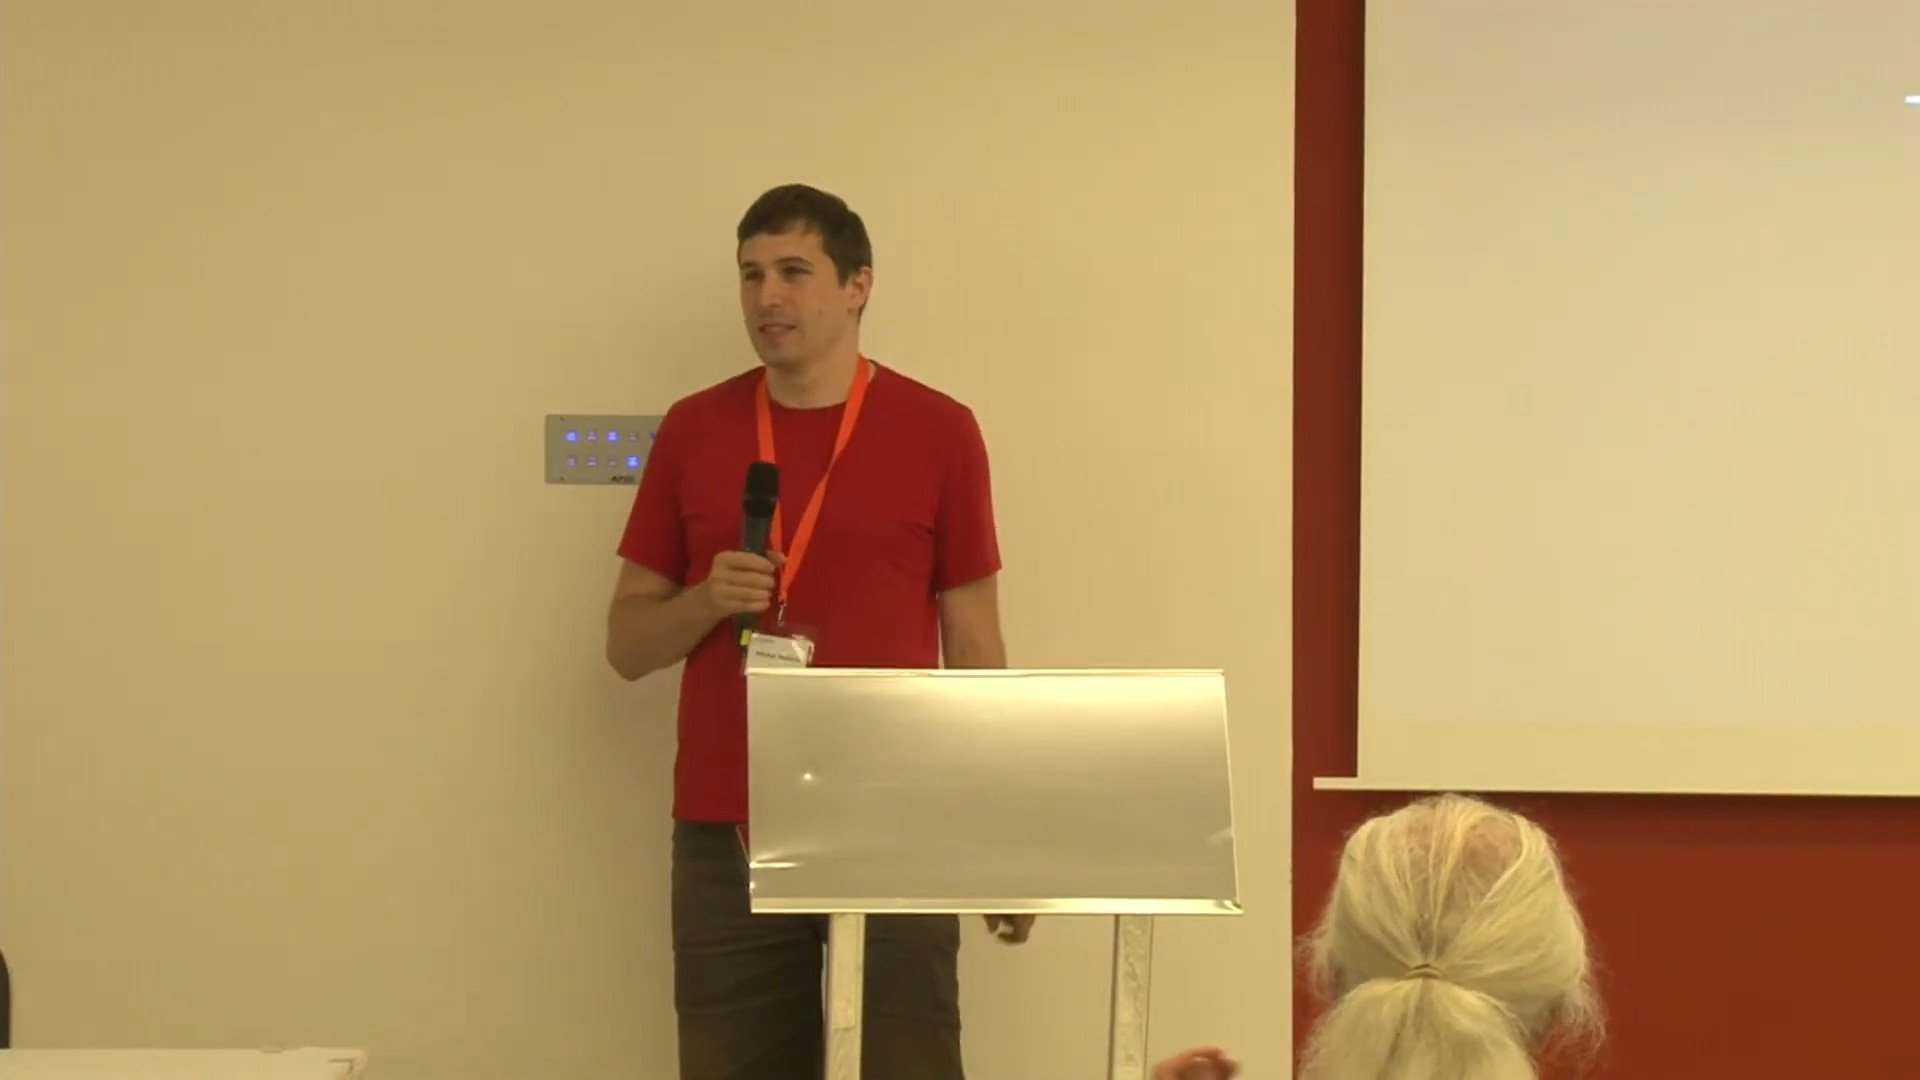
\includegraphics[width=\linewidth]{figs/michal-po-prednasce}\par\medskip
\fboxsep=0pt\kern-\fboxrule\relax\fbox{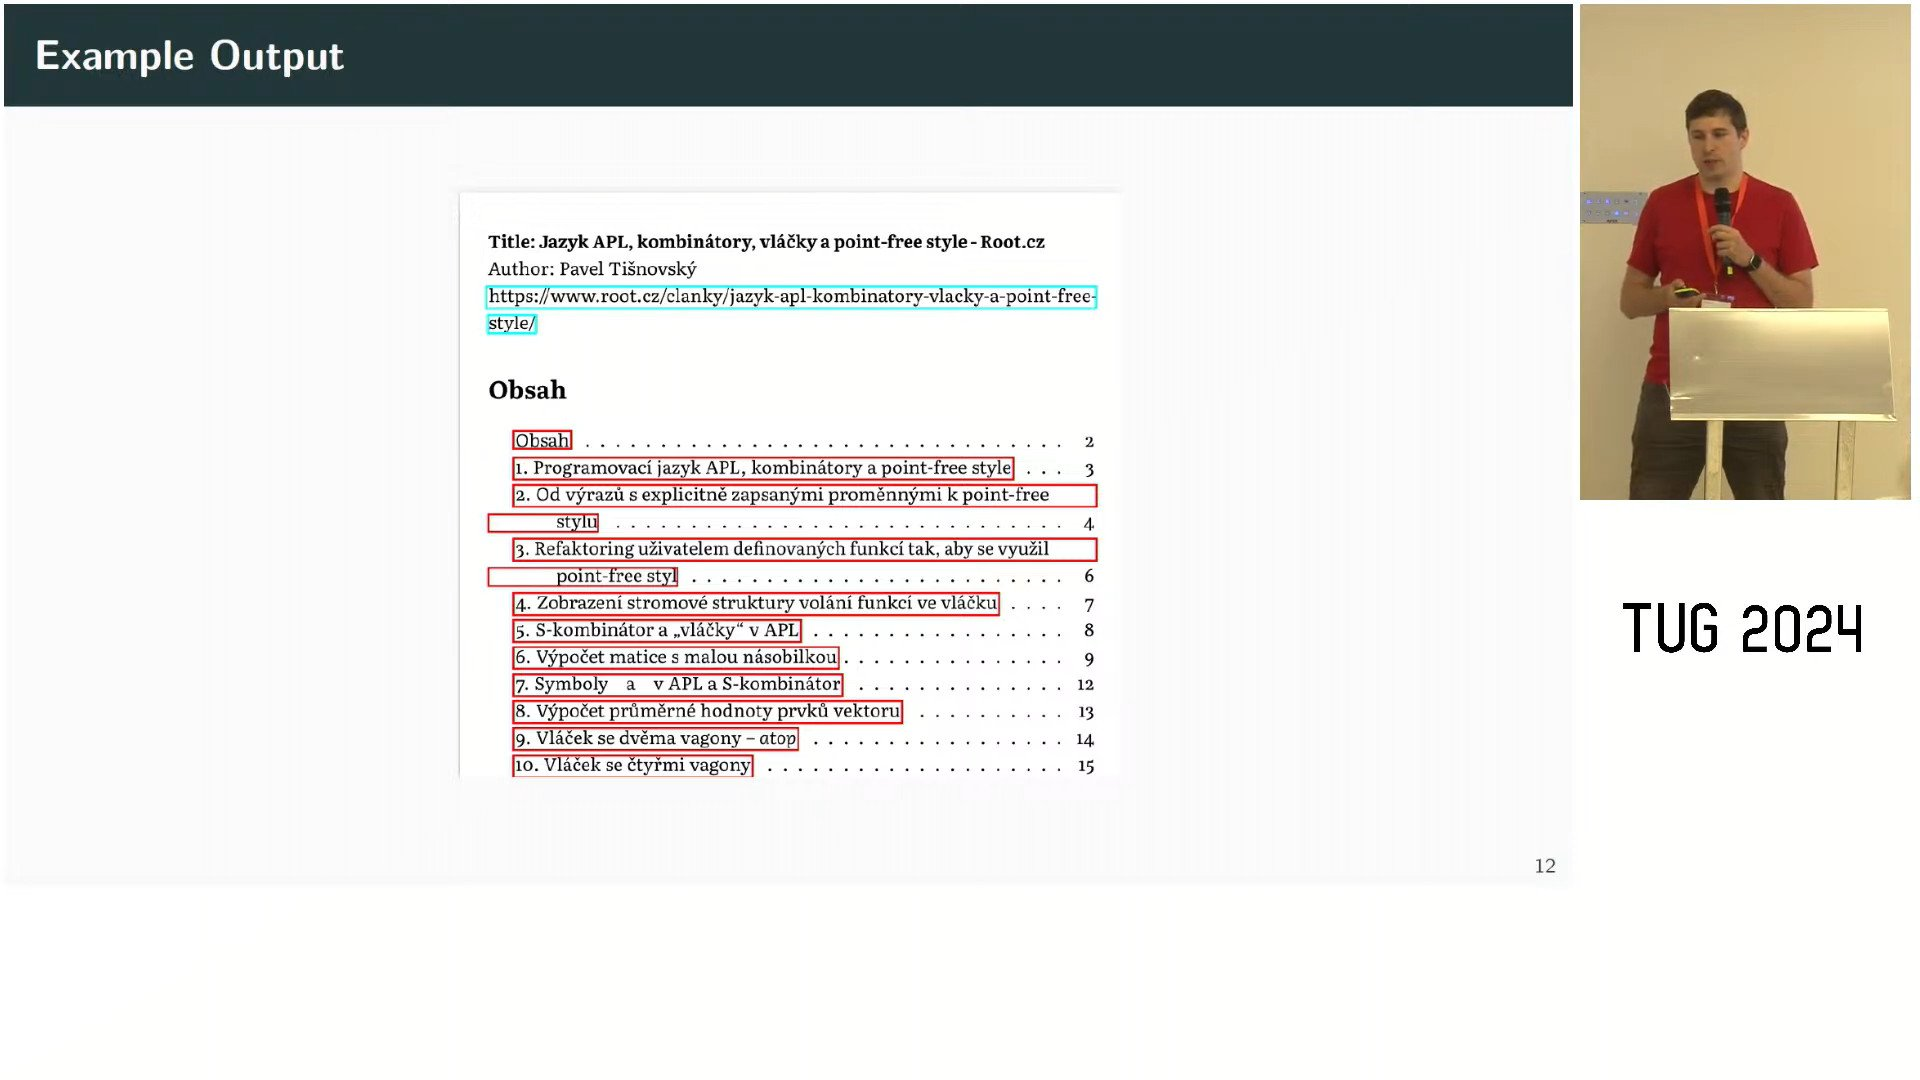
\includegraphics[width=\linewidth]{figs/michal-behem-prednasky}}%
\caption{Michal Hoftich přednáší o sazbě webových stránek pomocí svého programu Rmodepdf.}
\label{fig:michal}
\end{figure}

Během nedělního programu, který vedl Petr Sojka, představil Ondřej Sojka novinky z projektu univerzálních vzorů dělení slov v přednášce nazvané \emph{\foreignlanguage{english}{Expanding hyphenation patterns across Slavic languages}}~\cite{sojka2024extendinga, sojka2024extendingc}, vizte Obrázek~\ref{fig:petr-a-ondra}. Pro pokrytí většího množství slovanských jazyků se Ondřej chystá použít mezireprezentaci textu v mezinárodní fonetické abecedě \acro{IPA}.
\medskip

Záznam všech 31 přednášek lze nalézt na \href{https://www.youtube.com/playlist?list=PLLt9mKFAx-FZCy6aqYbXSNyaAkr8Nv14X}{kanálu YouTube \acro{TUG}u}~\cite{youtube}.
Program konference zakončil varhanní koncert barokních skladeb v kostele U Salvátora. 
% pamatujete si někdo jméno toho varhaníka? nikde ho nemůžu dohledat.

\begin{figure}[p]
\centering
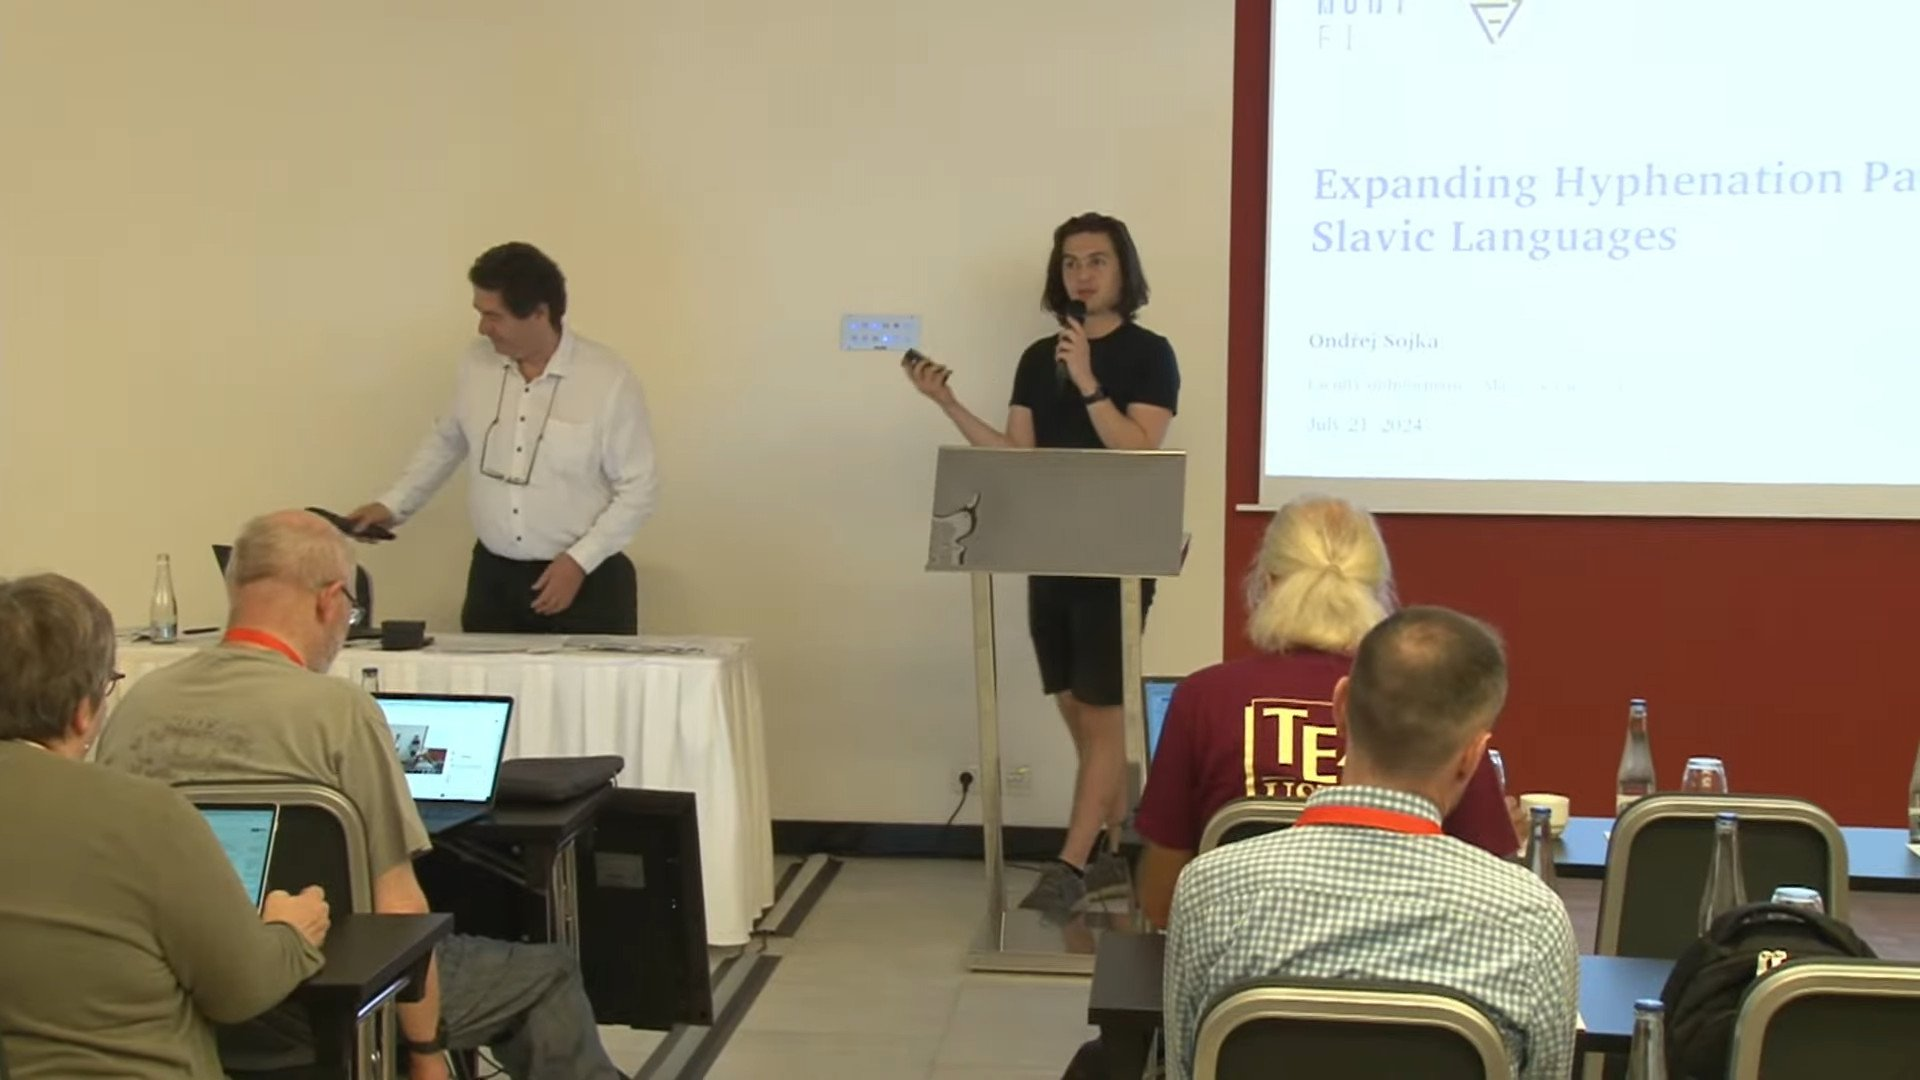
\includegraphics[width=\linewidth]{figs/petr-a-ondra-pred-prednaskou}\par\medskip
\fboxsep=0pt\kern-\fboxrule\relax\fbox{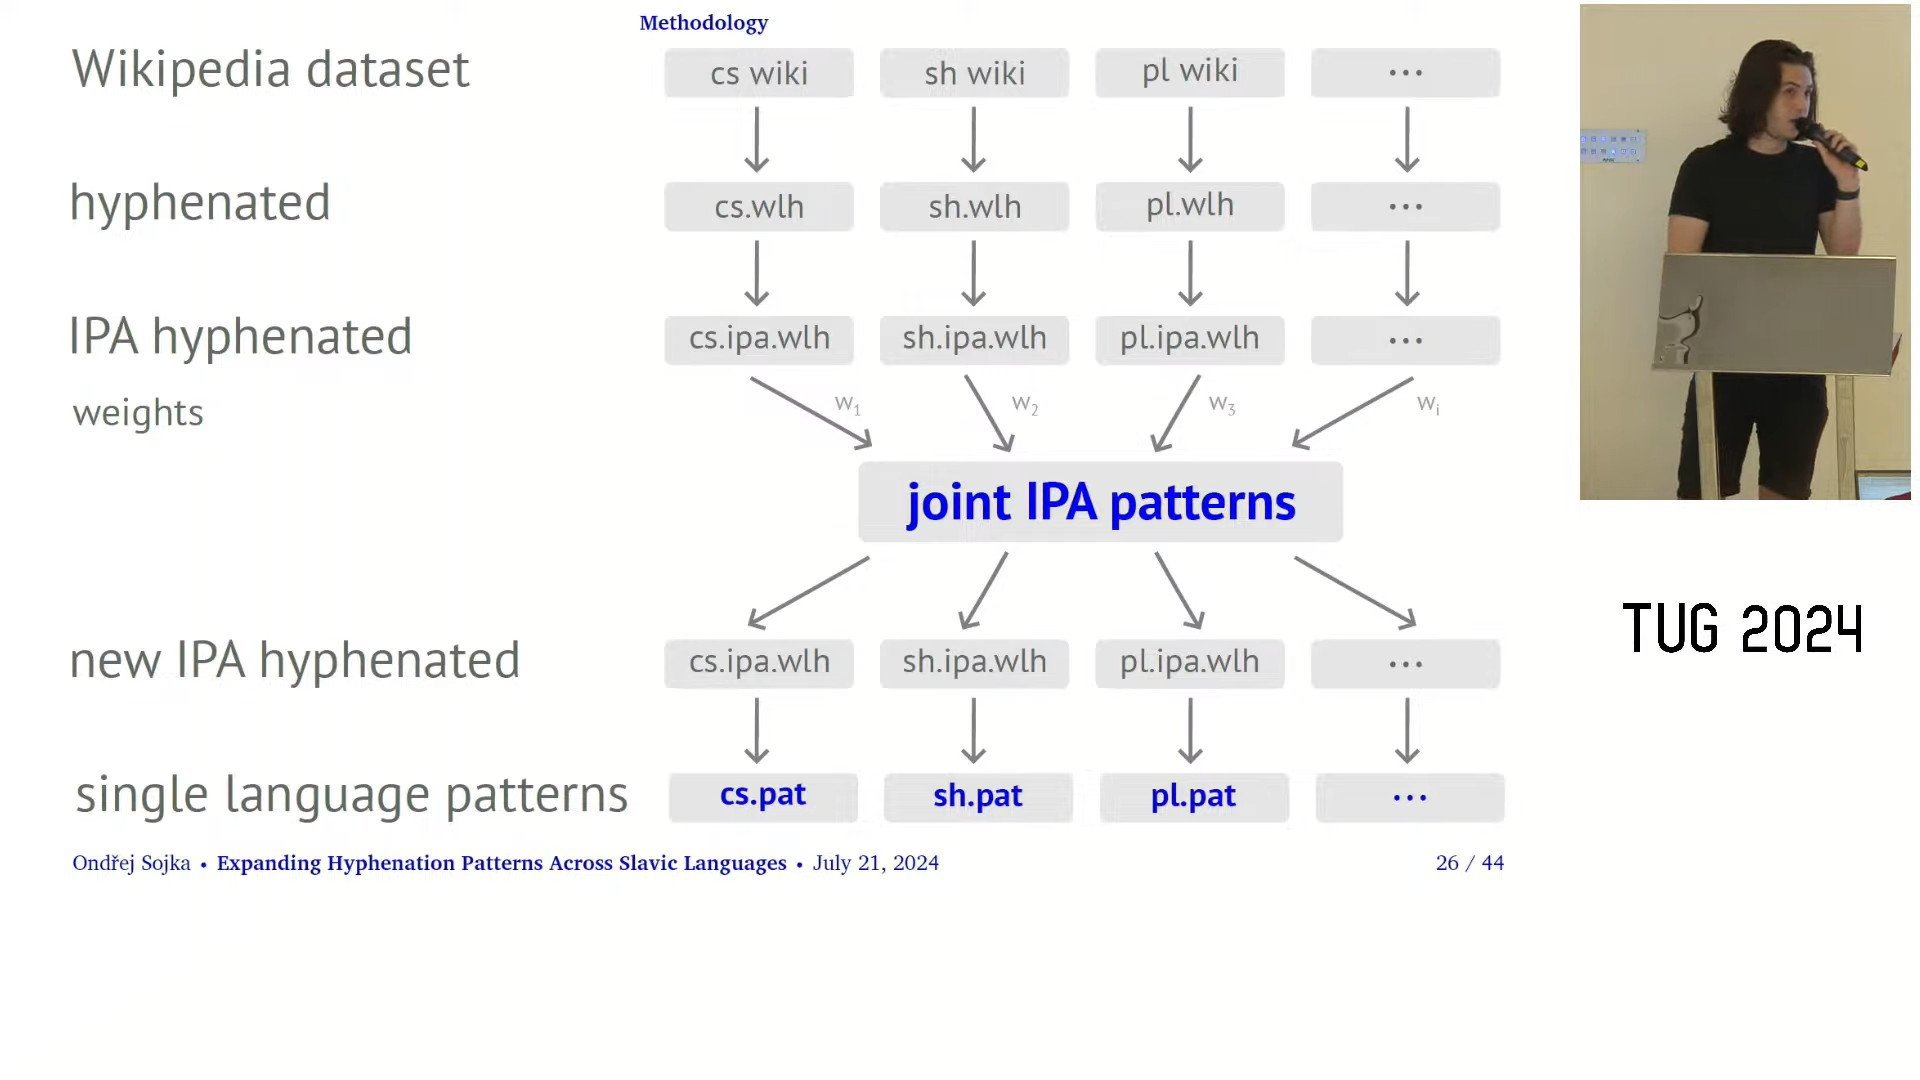
\includegraphics[width=\linewidth]{figs/ondra-behem-prednasky}}%
\caption{Ondřej Sojka přednáší o přípravě panslovanských vzorů dělení slov pomocí mezinárodní fonetické abecedy \acro{IPA}.}
\label{fig:petr-a-ondra}
\end{figure}

\begin{figure}[p]
\centering
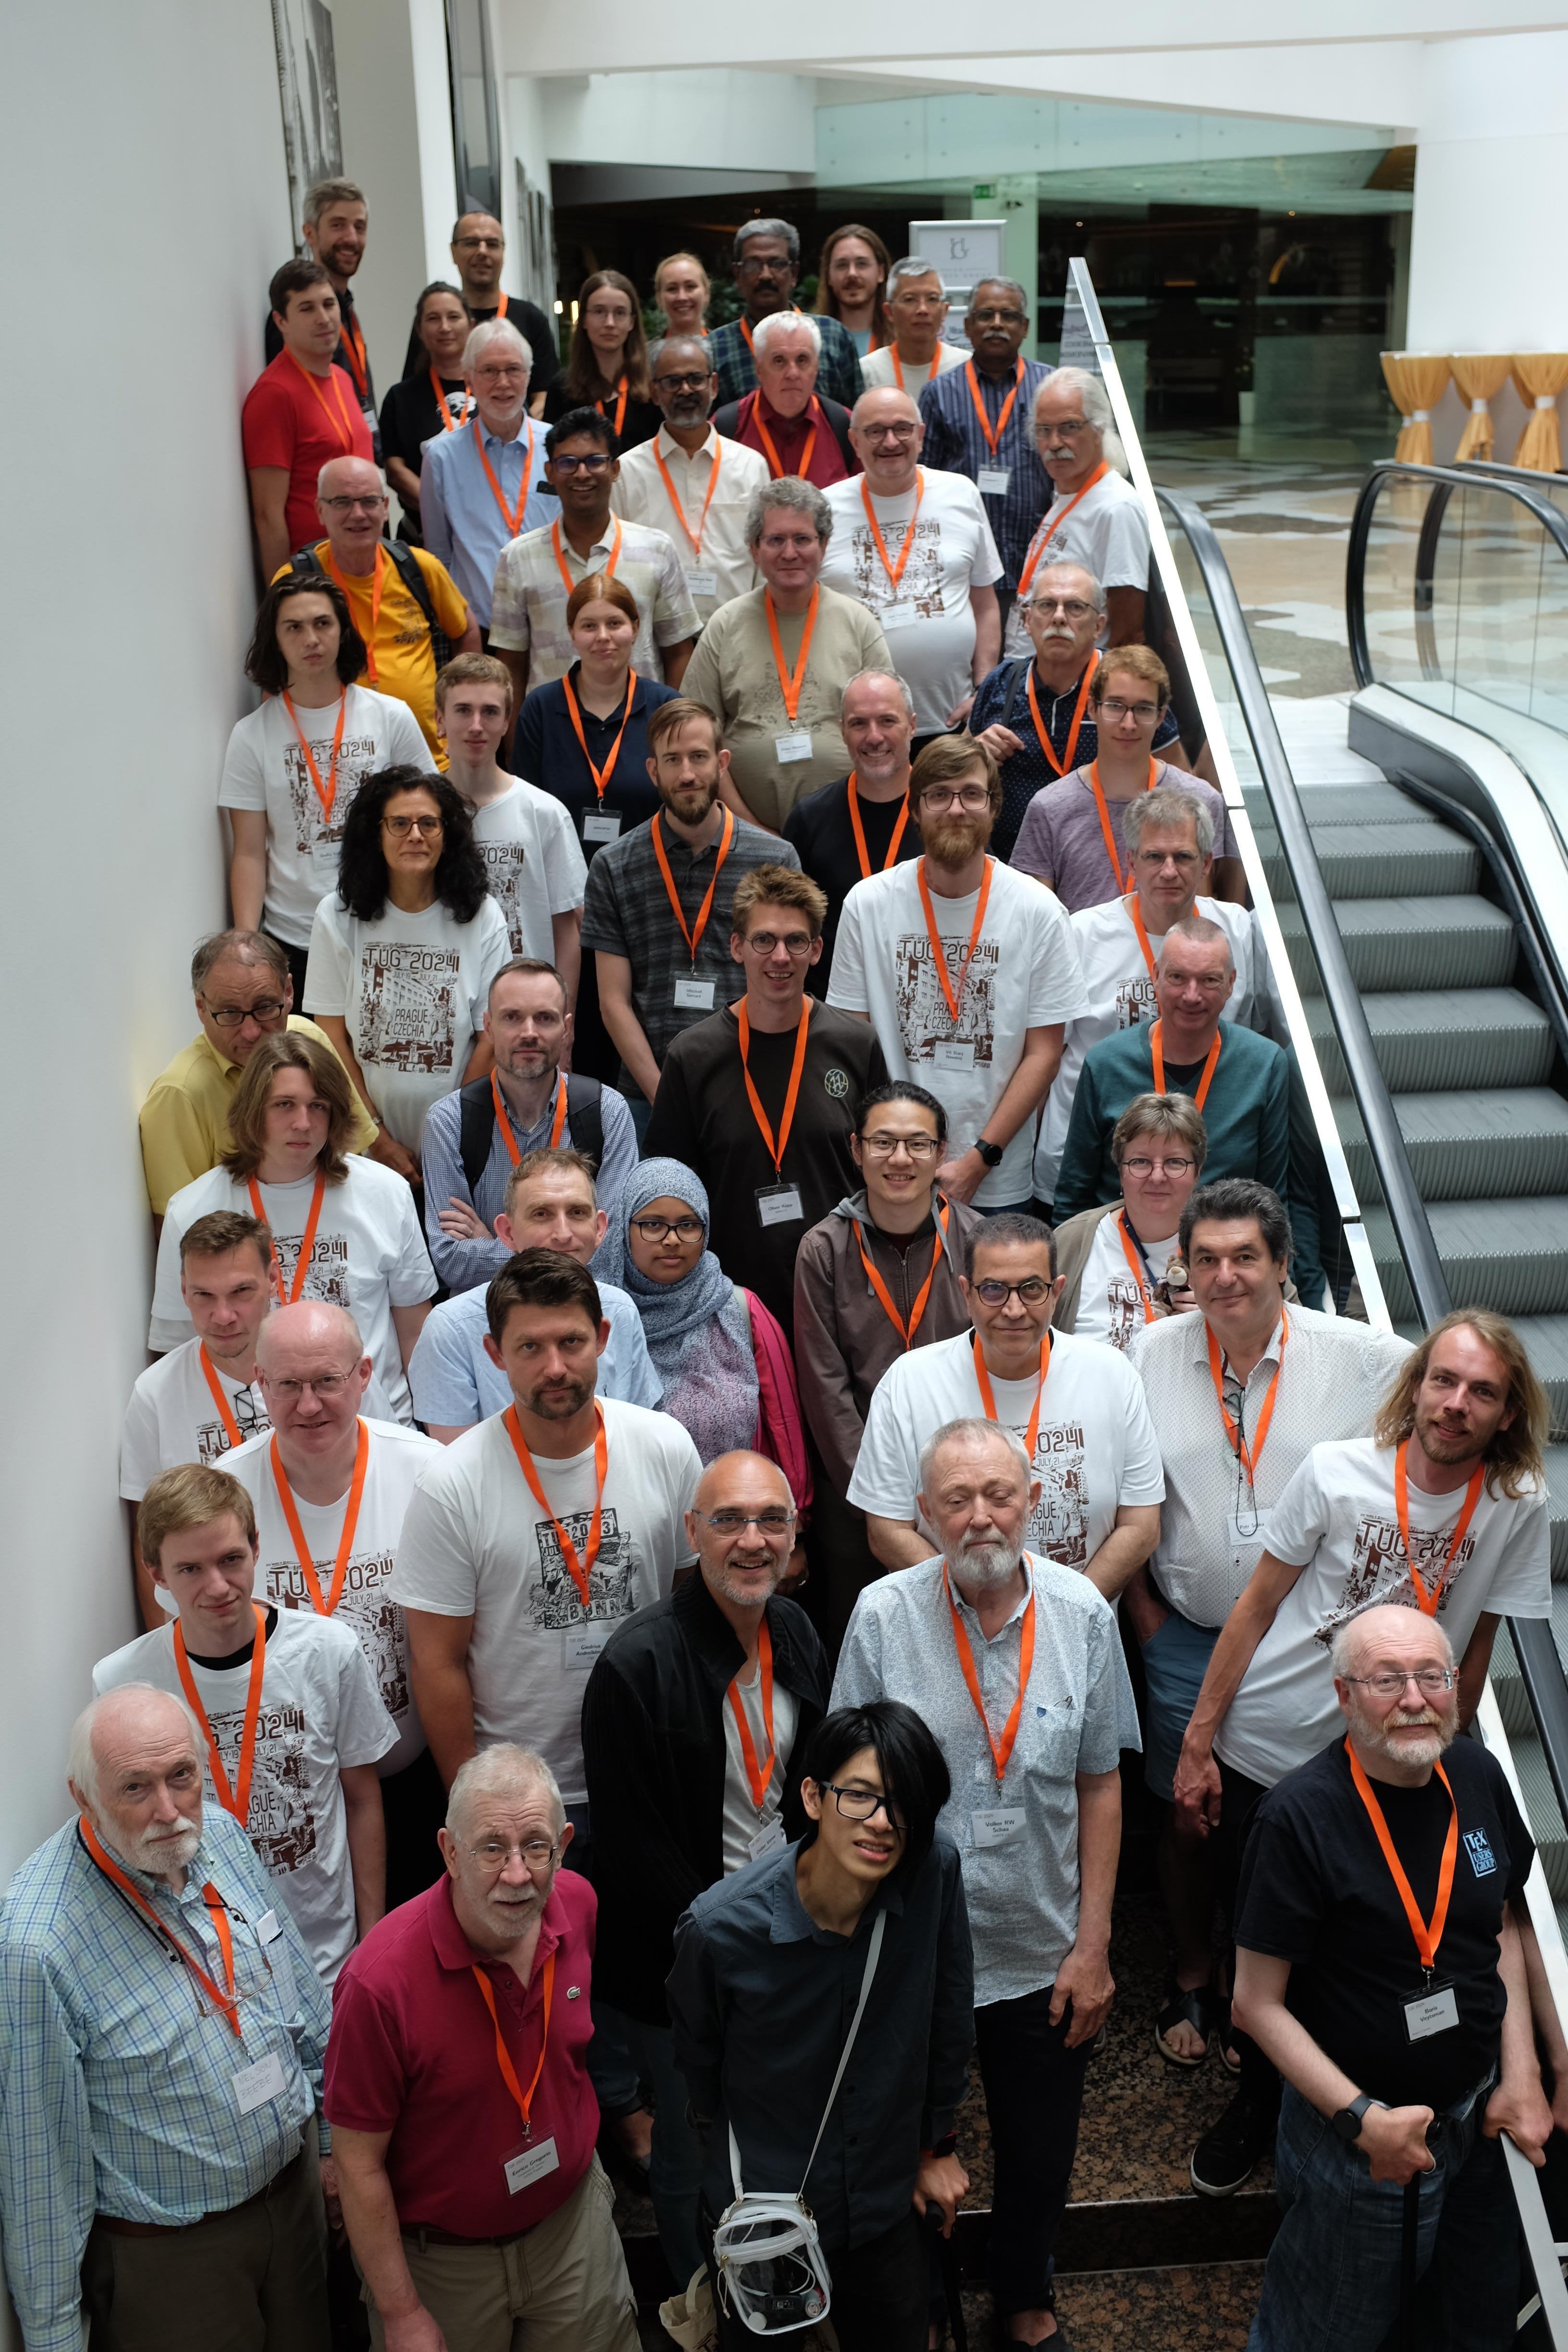
\includegraphics[width=0.9\linewidth]{figs/tug24-group-photo}%
\caption{Skupinová fotografie účastníků konference.}
\end{figure}

\begingroup
\sloppy
\printbibliography
\endgroup

\begin{summary}
This article reports on the participation of \CSTUG{} members at TUG 2024 in Prague.
\end{summary}
\end{document}
